% ============================================================
%  Příprava na maturitu – Elektrotechnika
%  Okruh 14: Napájecí zdroje, akumulátory a záložní zdroje
% ============================================================

\documentclass[a4paper,10pt]{article}

\usepackage[T1]{fontenc}
\usepackage[utf8]{inputenc}
\usepackage[left=2.0cm, right=1.8cm, top=1.8cm, bottom=1.8cm]{geometry}
\usepackage{parskip}
\usepackage{xcolor}
\usepackage{tabularx}
\usepackage{booktabs}
\usepackage{tikz}
\usepackage{mdframed}
\usepackage{amsmath}
\usepackage{enumitem}
\usepackage{circuitikz}

\usetikzlibrary{arrows.meta, positioning, decorations.pathmorphing, shapes.geometric, calc}

% --- Barvy ---
\definecolor{accent}{HTML}{1A3A5C}
\definecolor{lightblue}{HTML}{EAF2F8}
\definecolor{lightyellow}{HTML}{FDFBE4}
\definecolor{lightgreen}{HTML}{EAF7EA}
\definecolor{lightred}{HTML}{FDE8E8}
\definecolor{lightgray}{HTML}{F4F4F4}

% --- Boxy ---
\newmdenv[backgroundcolor=lightblue,linecolor=accent!40,roundcorner=4pt,
  innertopmargin=6pt,innerbottommargin=6pt,innerleftmargin=8pt,innerrightmargin=8pt]{pojmybox}
\newmdenv[backgroundcolor=lightyellow,linecolor=accent!30,roundcorner=4pt,
  innertopmargin=6pt,innerbottommargin=6pt,innerleftmargin=8pt,innerrightmargin=8pt]{vysvetlenibox}
\newmdenv[backgroundcolor=lightgreen,linecolor=accent!40,roundcorner=4pt,
  innertopmargin=6pt,innerbottommargin=6pt,innerleftmargin=8pt,innerrightmargin=8pt]{vzorcebox}
\newmdenv[backgroundcolor=lightred,linecolor=accent!30,roundcorner=4pt,
  innertopmargin=6pt,innerbottommargin=6pt,innerleftmargin=8pt,innerrightmargin=8pt]{durazbox}

\setlist[itemize]{noitemsep, leftmargin=1.4em, topsep=2pt}
\setlist[enumerate]{noitemsep, leftmargin=1.4em, topsep=2pt}

% --- Zkratka pro jednotky ---
\newcommand{\jednotka}[1]{\,[\mathrm{#1}]}

\begin{document}

% ============================================================
\section*{\large Okruh 14 – Napájecí zdroje, akumulátory a záložní zdroje}

\begin{pojmybox}
\textbf{Klíčové pojmy:}
lineární zdroj, spínaný zdroj (SMPS), usměrňovač, Graetzův můstek, filtrace (vyhlazení), stabilizátor (LDO), akumulátor (Pb, Li-Ion), kapacita baterie, BMS, záložní zdroj (UPS), offline / online UPS, střídač
\end{pojmybox}

\begin{vysvetlenibox}

% ================================================================
\subsection*{1. Blokové schéma klasického (lineárního) zdroje}

Většina elektroniky (PC, TV, telefony) potřebuje ke své funkci malé **stejnosměrné napětí (DC)**, např. 5V nebo 12V. V zásuvce je ale **střídavé napětí (AC)** 230V. Změna AC na DC probíhá v několika krocích:

\begin{center}
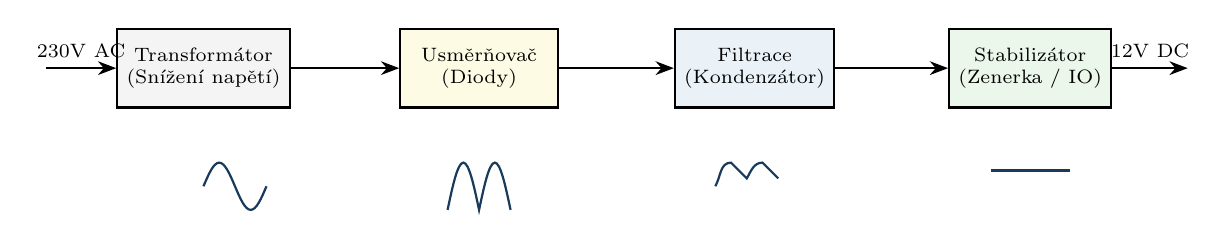
\begin{tikzpicture}[>=Stealth, font=\scriptsize, thick]
  % Bloky
  \node[draw, fill=lightgray, minimum width=2cm, minimum height=1cm, align=center] (trafo) at (0,0) {Transformátor\\(Snížení napětí)};
  \node[draw, fill=lightyellow, minimum width=2cm, minimum height=1cm, align=center] (rect) at (3.5,0) {Usměrňovač\\(Diody)};
  \node[draw, fill=lightblue, minimum width=2cm, minimum height=1cm, align=center] (filt) at (7,0) {Filtrace\\(Kondenzátor)};
  \node[draw, fill=lightgreen, minimum width=2cm, minimum height=1cm, align=center] (stab) at (10.5,0) {Stabilizátor\\(Zenerka / IO)};
  
  % Šipky
  \draw[->] (-2,0) -- (trafo) node[midway, above] {230V AC};
  \draw[->] (trafo) -- (rect);
  \draw[->] (rect) -- (filt);
  \draw[->] (filt) -- (stab);
  \draw[->] (stab) -- (12.5,0) node[midway, above] {12V DC};

  % Průběhy napětí pod bloky
  % Trafo (malá sinusovka)
  \draw[accent] (0,-1.5) sin (0.2,-1.2) cos (0.4,-1.5) sin (0.6,-1.8) cos (0.8,-1.5);
  % Usměrňovač (pulzující DC)
  \draw[accent] (3.1,-1.8) sin (3.3,-1.2) cos (3.5,-1.8) sin (3.7,-1.2) cos (3.9,-1.8);
  % Filtrace (zvlněné DC)
  \draw[accent] (6.5,-1.5) to[out=60, in=180] (6.7,-1.2) -- (6.9,-1.4) to[out=60, in=180] (7.1,-1.2) -- (7.3,-1.4);
  % Stabilizátor (rovná čára)
  \draw[accent, line width=1.2pt] (10.0,-1.3) -- (11.0,-1.3);
\end{tikzpicture}
\end{center}

% ================================================================
\subsection*{2. Usměrňovače}

Převádějí střídavý proud (měnící směr) na stejnosměrný (pulzující v jednom směru) využitím diod (\textit{viz Okruh 12}).

\textbf{A) Jednocestný usměrňovač:} Používá jen jednu diodu. Propustí jen kladnou půlvlnu, zápornou odřízne. Velmi neefektivní (obrovské zvlnění).

\textbf{B) Dvoucestný (Graetzův) můstek:} Používá **4 diody**. „Překlopí“ zápornou půlvlnu do kladné, takže využívá celou energii střídavého proudu.
Když je na horním vstupu (+), proud teče přes D1, zátěží dolů a přes D3 zpět. Když se polarita otočí, proud teče přes D2, zátěží opět dolů a přes D4 zpět. \textbf{Zátěží teče proud vždy stejným směrem!}

\begin{center}
\begin{circuitikz}[font=\small, thick]
  % Vstup AC
  \draw (-2, 1.5) to[sinusoidal voltage source, l=AC Vstup] (-2, -1.5);
  \draw (-2, 1.5) -- (0, 1.5);
  \draw (-2, -1.5) -- (0, -1.5);
  
  % Můstek
  \draw (0, 1.5) to[Do, l_=D1, *-*] (2, 0);
  \draw (0, -1.5) to[Do, l=D2, *-*] (2, 0);
  \draw (-2, 0) to[Do, l=D3, *-*] (0, -1.5);
  \draw (-2, 0) to[Do, l_=D4, *-*] (0, 1.5);
  
  % Připojení k uzlům
  \draw (0,1.5) -- (0,1.5); % horní
  \draw (0,-1.5) -- (0,-1.5); % dolní
  \draw (-2,0) -- (-2,0); % levý - POZOR křížení bez vodivého spoje!
  \draw[dashed, gray] (-1, 1.5) arc (0:180:0.2); % náznak přeskočení, v circuitikz se často kreslí uzel, my to propojili jasně.
  
  % Výstup
  \draw (2, 0) -- (4, 0) node[right, red] {+ DC};
  \draw (-2, 0) -- (-2, 2.5) -- (4, 2.5) node[right, blue] {$-$ DC};
  
  % Filtrační kondenzátor a zátěž
  \draw (3, 2.5) to[eC, l=$C_{filtr}$, *-*] (3, 0);
  \draw (4, 2.5) to[R, l=$R_{z\acute{a}t\check{e}\check{z}}$] (4, 0);
\end{circuitikz}
\end{center}

% ================================================================
\subsection*{3. Lineární vs. Spínaný zdroj (SMPS)}

\begin{center}
\begin{tabularx}{0.97\linewidth}{@{} l X X @{}}
\toprule
\textbf{Vlastnost} & \textbf{Lineární zdroj (Klasický)} & \textbf{Spínaný zdroj (SMPS)} \\
\midrule
\textbf{Princip} & Velké trafo sníží AC, pak se usměrní. Přebytečné napětí se "spálí" na teplo na stabilizátoru. & 230V se ihned usměrní, "rozseká" tranzistorem na vysokou frekvenci (kHz), prožene malinkým trafem a usměrní. \\
\textbf{Rozměry a váha} & Těžký a velký (obří železné trafo). & Velmi lehký a malý. \\
\textbf{Účinnost} & Nízká (často kolem 40 - 50 \%). & Velmi vysoká (85 - 95 \%). \\
\textbf{Nevýhody} & Hřeje. & Složitý obvod, generuje vysokofrekvenční rušení. \\
\textbf{Typické použití} & Hi-Fi audio zesilovače (čistý proud), laboratoře. & Nabíječky na mobily, zdroje v PC, adaptéry k notebookům. \\
\bottomrule
\end{tabularx}
\end{center}

% ================================================================
\subsection*{4. Akumulátory (Sekundární články)}

Reverzibilní zdroje napětí (lze je nabíjet - dodáním el. energie se obnoví chemické složení). \textbf{Kapacita} se udává v ampérhodinách [Ah] nebo [mAh] (baterie 2000 mAh dokáže dodávat proud 2000 mA po dobu 1 hodiny).

\begin{itemize}
    \item \textbf{Olověný akumulátor (Pb):} $2\,\mathrm{V}$ na článek (autobaterie = 6 článků v sérii = 12 V). Těžký, odolný proti velkým proudům (startování auta), nesmí se hluboce vybít, jinak sulfatuje a zničí se.
    \item \textbf{Lithium-Iontový (Li-Ion / Li-Pol):} $3{,}6\,\mathrm{V}$ až $3{,}7\,\mathrm{V}$ na článek. Obrovská hustota energie (mobily, elektromobily). Nemá paměťový efekt. 
\end{itemize}

\begin{durazbox}
\textbf{Ochrana Li-Ion (BMS - Battery Management System):}
Li-Ion články jsou extrémně nebezpečné při přebití (hrozí požár/výbuch) a zničí se při podbití (pod 2,5 V). Každá Li-Ion baterie proto **musí obsahovat BMS** – elektronický obvod, který neustále hlídá napětí, proud a teplotu každého článku a v případě nebezpečí jej odpojí (balancování článků).
\end{durazbox}

% ================================================================
\subsection*{5. Záložní zdroje (UPS - Uninterruptible Power Supply)}

Zajišťují nepřetržité napájení důležitých spotřebičů (servery, nemocnice) při výpadku sítě.

\textbf{A) Offline (Line-Interactive) UPS:}
Za normálního stavu je spotřebič napájen přímo ze sítě. Při výpadku elektronika přepne relé na napájení z baterie přes **střídač (Invertor)**, který dělá z 12V/24V DC opět 230V AC. \textit{Nevýhoda: Přepnutí trvá pár milisekund, občas propustí rušení ze sítě.}

\textbf{B) Online UPS (S dvojitou konverzí):}
Spotřebič je **neustále** napájen ze střídače (baterie). Neexistuje žádná doba přepnutí, spotřebič nepozná výpadek. Poskytuje naprosto čisté a dokonalé napětí nezávisle na kvalitě sítě. \textit{Použití: Kritická IT infrastruktura, serverovny.}

\begin{center}
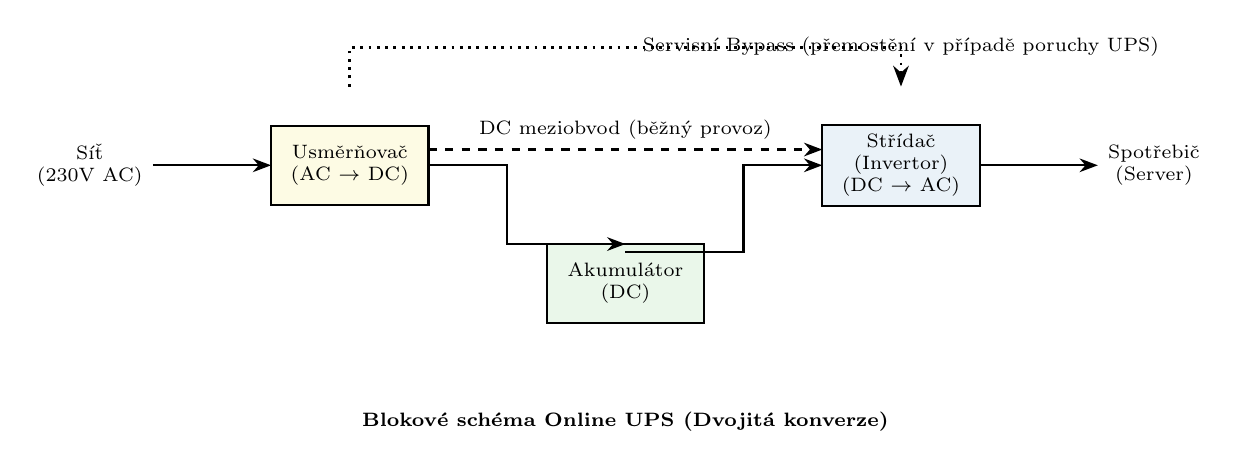
\begin{tikzpicture}[>=Stealth, font=\scriptsize, thick]
  % Síť
  \node[left, align=center] at (-1.5, 1) {Síť\\(230V AC)};
  \draw[->] (-1.5,1) -- (0,1);

  % Usměrňovač
  \node[draw, fill=lightyellow, minimum width=2cm, minimum height=1cm, align=center] (rect) at (1,1) {Usměrňovač\\(AC $\rightarrow$ DC)};
  
  % Baterie
  \node[draw, fill=lightgreen, minimum width=2cm, minimum height=1cm, align=center] (bat) at (4.5,-0.5) {Akumulátor\\(DC)};
  
  % Střídač
  \node[draw, fill=lightblue, minimum width=2cm, minimum height=1cm, align=center] (inv) at (8,1) {Střídač\\(Invertor)\\ (DC $\rightarrow$ AC)};

  % Výstup
  \draw[->] (9,1) -- (10.5,1) node[right, align=center] {Spotřebič\\(Server)};

  % Propojení DC sběrnice
  \draw[->] (2,1) -- (3,1) -- (3,0) -- (4.5,0); % do baterie (nabíjení)
  \draw[->] (4.5,-0.1) -- (6,-0.1) -- (6,1) -- (7,1); % z baterie do střídače
  \draw[->, dashed] (2,1.2) -- (7,1.2) node[midway, above] {DC meziobvod (běžný provoz)};

  % Bypass
  \draw[->, dotted, line width=1pt] (1,2) -- (1,2.5) -- (8,2.5) -- (8,2) node[midway, above] {Servisní Bypass (přemostění v případě poruchy UPS)};

  \node[below] at (4.5, -2) {\textbf{Blokové schéma Online UPS (Dvojitá konverze)}};
\end{tikzpicture}
\end{center}

\end{vysvetlenibox}

\end{document}